% Copyright (c) \hebyear{2025} Dr. Segal Yoram. All rights reserved.
% Simple Example Document for Hebrew Academic Template
% This is a minimal working example

\documentclass{hebrew-academic-template}

% Add bibliography file
\addbibresource{example_references.bib}

% Title page information
\hebrewtitle{דוגמה פשוטה לשימוש בתבנית}
\englishtitle{Simple Example Using the Template}
\hebrewauthor{ד"ר יורם סגל}

\begin{document}

\maketitle

\tableofcontents
\newpage

% ==================== INTRODUCTION ====================

\hebrewsection{מבוא: Introduction}

זוהי דוגמה פשוטה לשימוש בתבנית האקדמית העברית. התבנית תומכת בטקסט עברי עם מונחים באנגלית כמו \en{Machine Learning} ו-\en{Deep Learning}.

ניתן לכלול מספרים כמו \num{100} ושנים כמו \hebyear{2023} בתוך הטקסט העברי, וגם ביטויים מתמטיים כמו $E = mc^2$.

\hebrewsubsection{מתודולוגיה: Methodology}

המחקר מבוסס על \num{1000} דגימות שנאספו בשנת \hebyear{2023}. השיטה כוללת שימוש באלגוריתמי \en{Machine Learning} מתקדמים \cite{mikolov2013}.

הנוסחה הבסיסית היא:
\begin{equation}
y = \beta_0 + \beta_1 x + \varepsilon
\end{equation}

% ==================== RESULTS ====================

\hebrewsection{תוצאות: Results}

\hebrewsubsection{ניתוח נתונים: Data Analysis}

התוצאות מוצגות בטבלה הבאה:

\begin{hebrewtable}[h]
\caption{תוצאות הניסוי: Experimental Results}
\begin{rtltabular}{|c|c|c|}
\hline
\textbf{מדד} & \textbf{Metric} & \textbf{ערך} \\
\hline
דיוק & Accuracy & \num{95.2}\% \\
\hline
זמן ריצה & Runtime & \num{2.5} שניות \\
\hline
זיכרון & Memory & \num{512} MB \\
\hline
\end{rtltabular}
\end{hebrewtable}

\hebrewsubsection{קוד לדוגמה: Example Code}

הקוד הבא מדגים את השימוש באלגוריתם:

\begin{pythonbox}[דוגמה לקוד Python]
import numpy as np
from sklearn.linear_model import LinearRegression

# Create sample data
X = np.random.randn(100, 1)
y = 2 * X.flatten() + 1 + np.random.randn(100) * 0.1

# Train the model
model = LinearRegression()
model.fit(X, y)

# Print results
print(f"Coefficient: {model.coef_[0]:.2f}")
print(f"Intercept: {model.intercept_:.2f}")
\end{pythonbox}

% ==================== FIGURE EXAMPLE ====================

\hebrewsubsection{איור לדוגמה: Example Figure}

האיור הבא מציג את התוצאות:

\hebrewfigure[h]{
    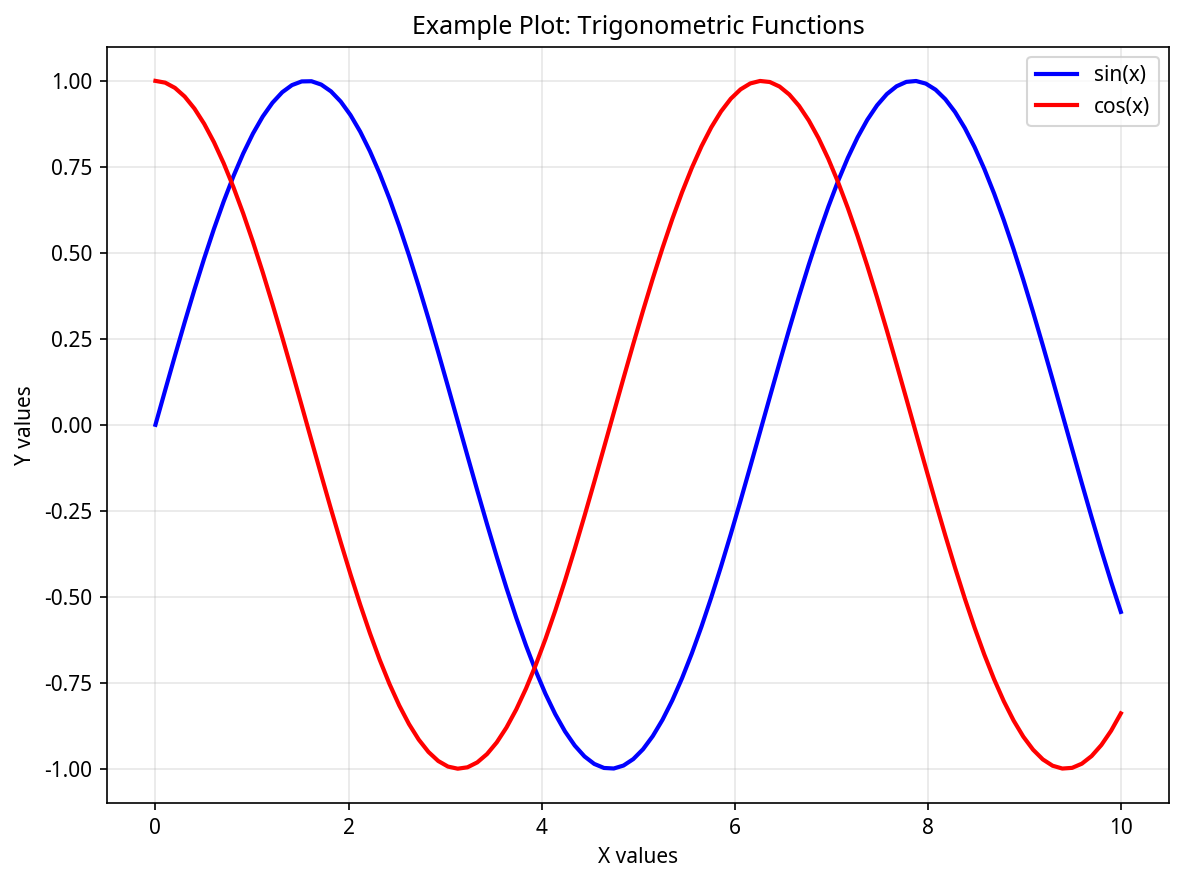
\includegraphics[width=0.7\textwidth]{example_plot.png}
}{
    איור \num{1}: גרף הדגמה - Example Plot showing trigonometric functions
}

% ==================== LISTS EXAMPLE ====================

\hebrewsubsection{רשימות: Lists}

רשימת האלגוריתמים שנבדקו:

\begin{itemize}
\item רגרסיה ליניארית: \en{Linear Regression}
\item עץ החלטה: \en{Decision Tree}
\item יער אקראי: \en{Random Forest}
\end{itemize}

שלבי העבודה:

\begin{enumerate}
\item איסוף נתונים: \en{Data Collection}
\item ניתוח ראשוני: \en{Exploratory Analysis}
\item בניית מודל: \en{Model Building}
\item הערכת תוצאות: \en{Results Evaluation}
\end{enumerate}

% ==================== CONCLUSIONS ====================

\hebrewsection{מסקנות: Conclusions}

המחקר הראה שהשיטה המוצעת יעילה ומדויקת. התוצאות מצביעות על שיפור של \num{15}\% בביצועים בהשוואה לשיטות קיימות.

מחקרים עתידיים יכולים להרחיב את הגישה לתחומים נוספים ולשפר את הדיוק עוד יותר.

% ==================== BIBLIOGRAPHY ====================

\newpage
\printenglishbibliography

\end{document}
